\documentclass{standalone}
\usepackage{tikz}

\begin{document}
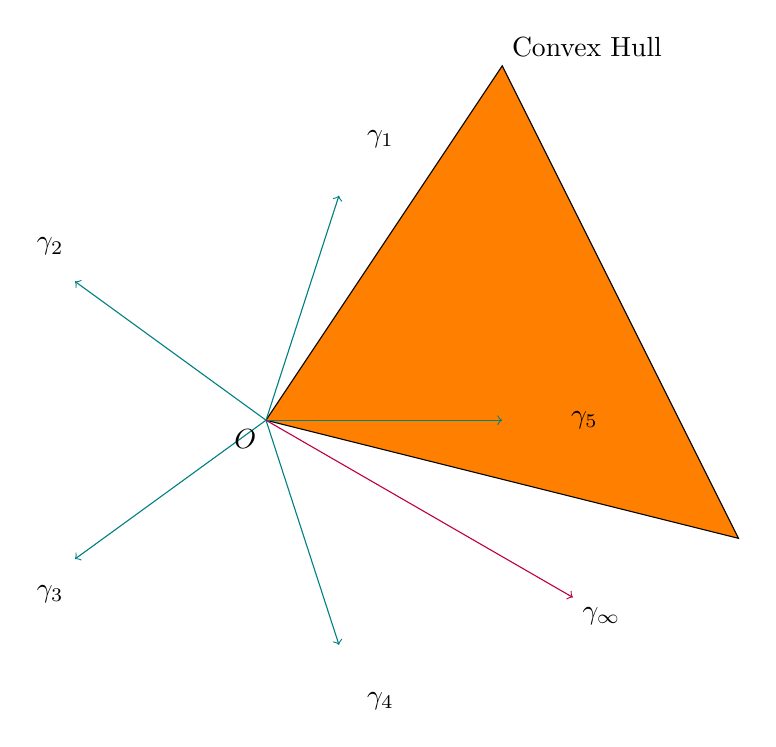
\begin{tikzpicture}[scale=1.5]
    % Define colors
    \colorlet{coupling}{teal}
    \colorlet{convex_hull}{orange}
    \colorlet{distance_vector}{purple}

    % Draw the convex hull
    \draw[fill=convex_hull] (0,0) -- (2,3) -- (4,-1) -- cycle;

    % Draw the coupling vectors
    \foreach \i in {1,...,5} {
        \pgfmathsetmacro{\angle}{72*\i}
        \draw[coupling,->] (0,0) -- (\angle:2);
    }

    % Draw the distance vector
    \draw[distance_vector,->] (0,0) -- (-30:3);

    % Label points and vectors
    \node at (0,0) [below left] {$O$};
    \node at (2,3) [above right] {Convex Hull};
    \node at (4,-1) {};
    \node at (-30:3) [below right] {$\gamma_\infty$};

    % Add labels for coupling vectors
    \foreach \i in {1,...,5} {
        \pgfmathsetmacro{\angle}{72*\i}
        \node at (\angle:2.5) [right] {$\gamma_{\i}$};
    }
\end{tikzpicture}
\end{document}